\begin{figure}[!t]
\centering
\begin{subfigure}{0.48\textwidth}
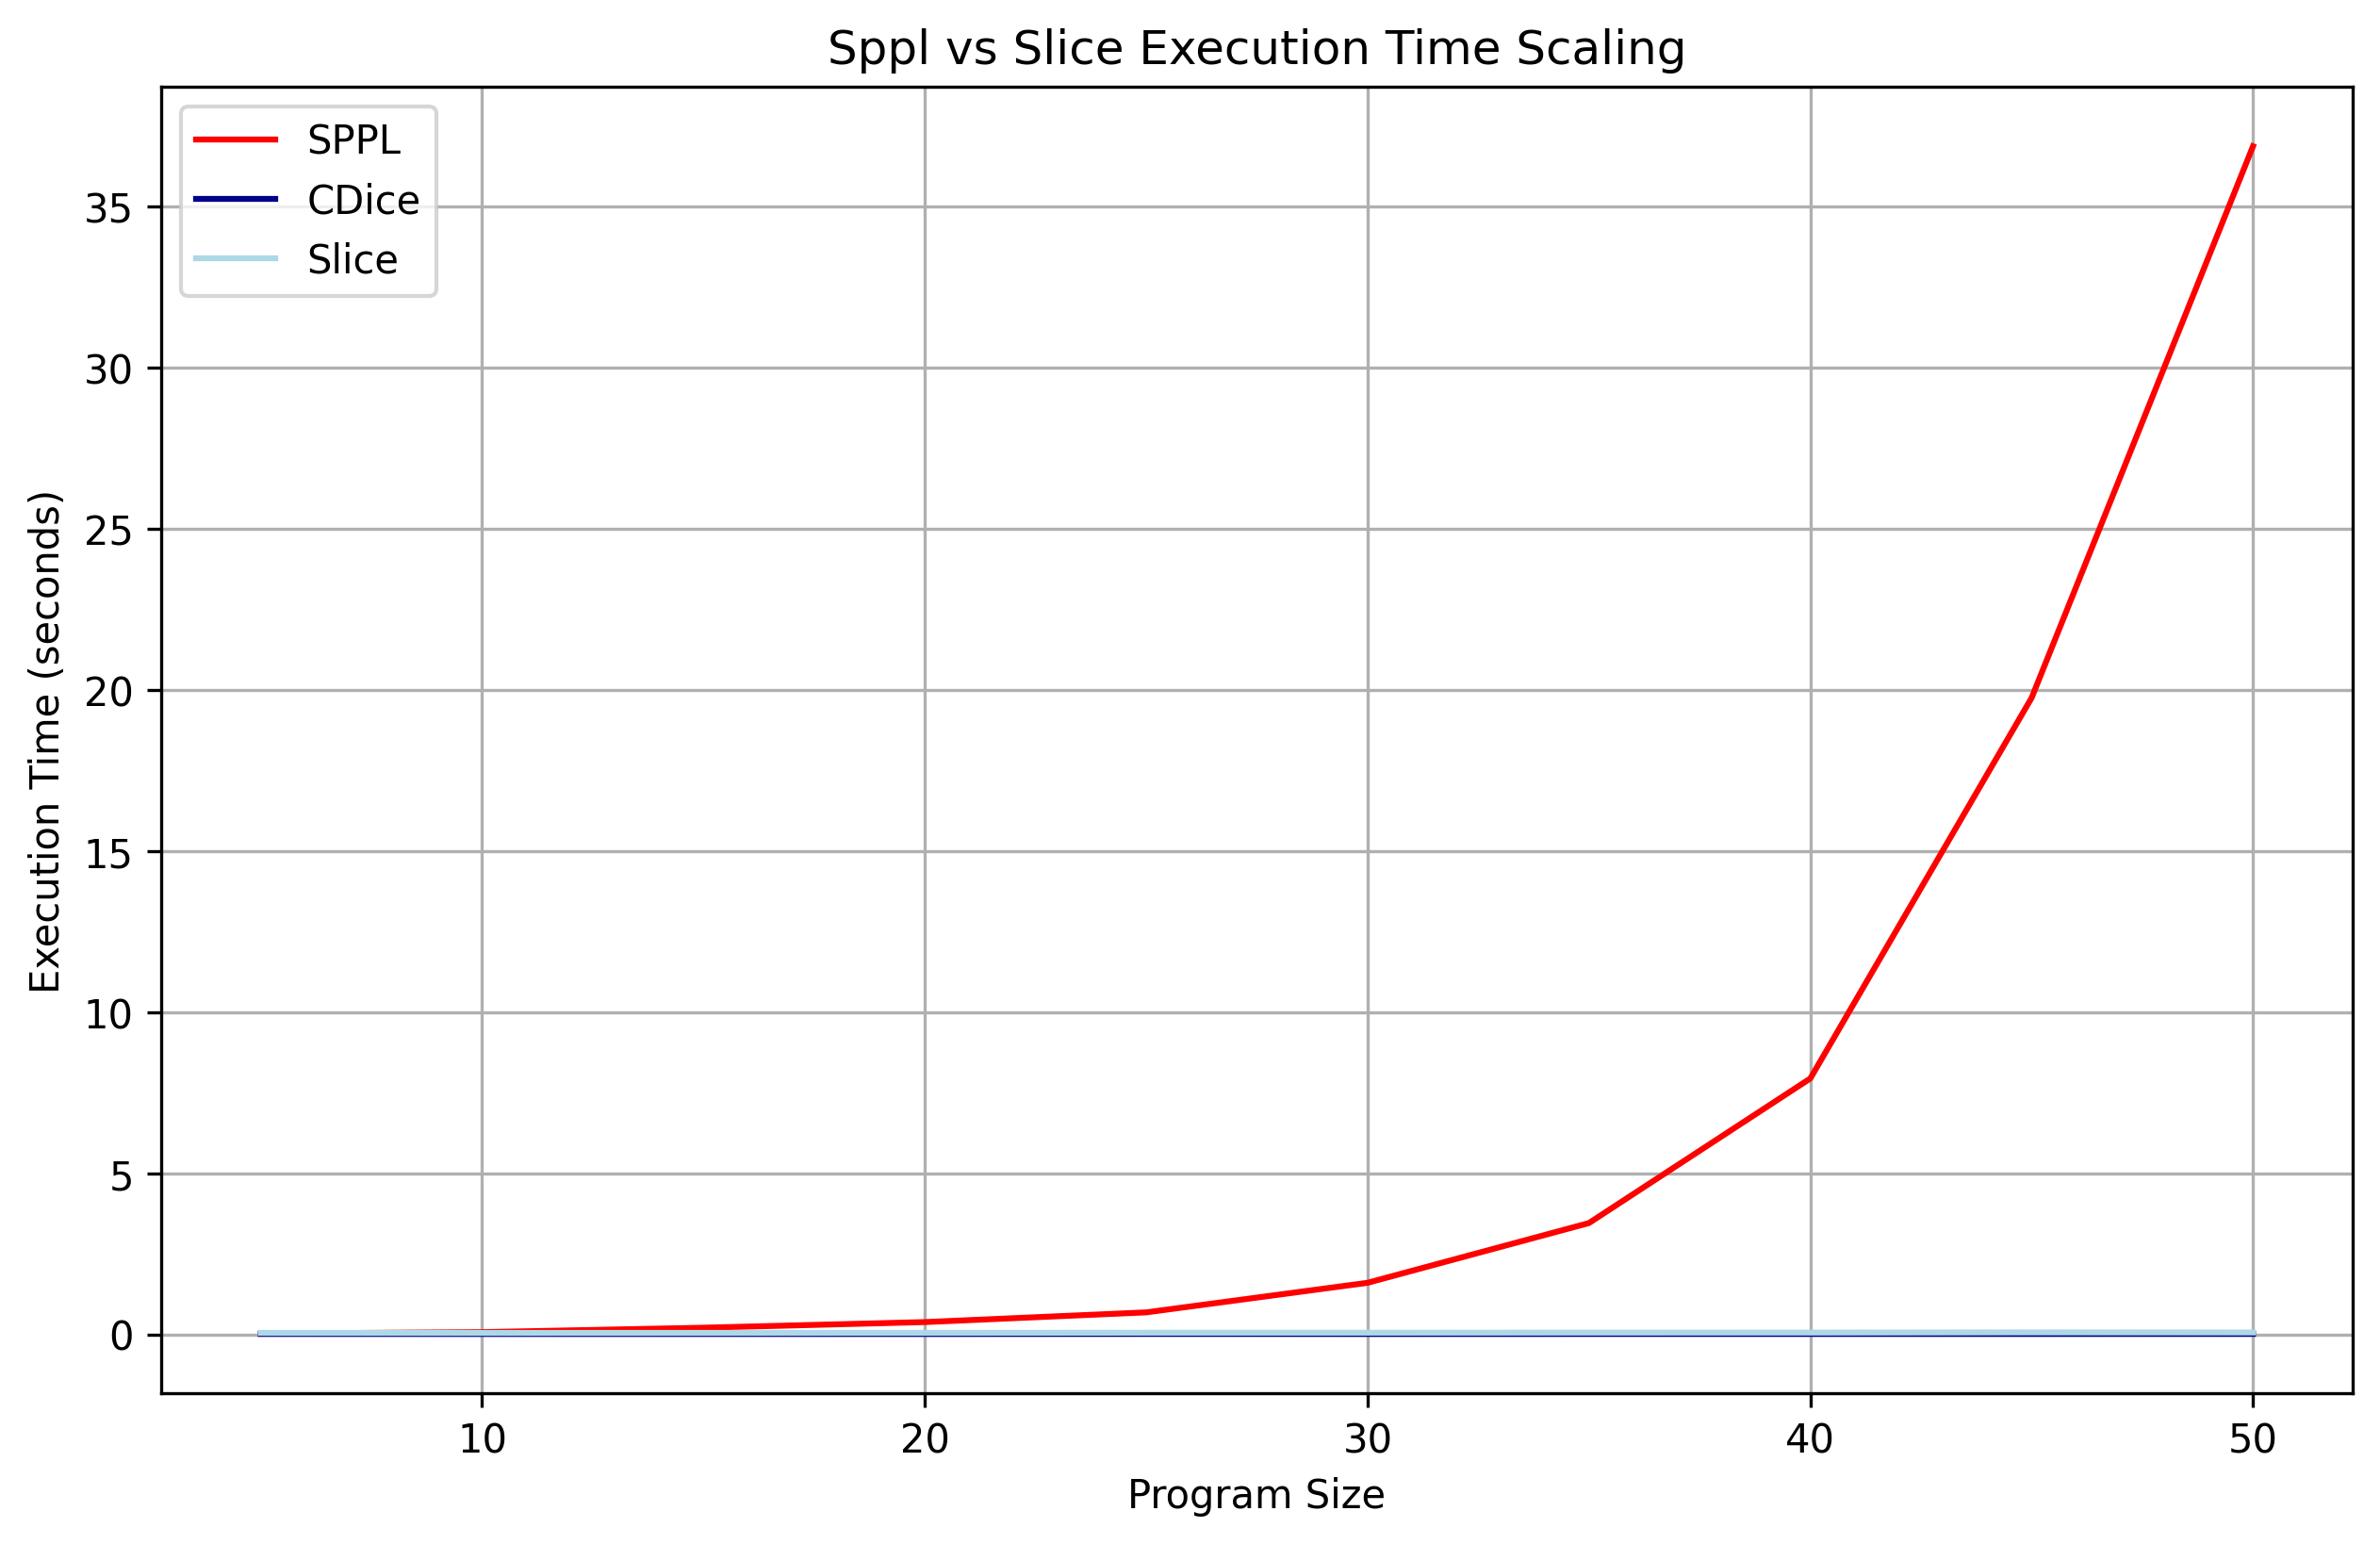
\includegraphics[width=\textwidth]{../images/scaling/build_alternating_guard_contdice_1.png}
\caption{Alternating Guard 1}
\end{subfigure}
\hfill
\begin{subfigure}{0.48\textwidth}
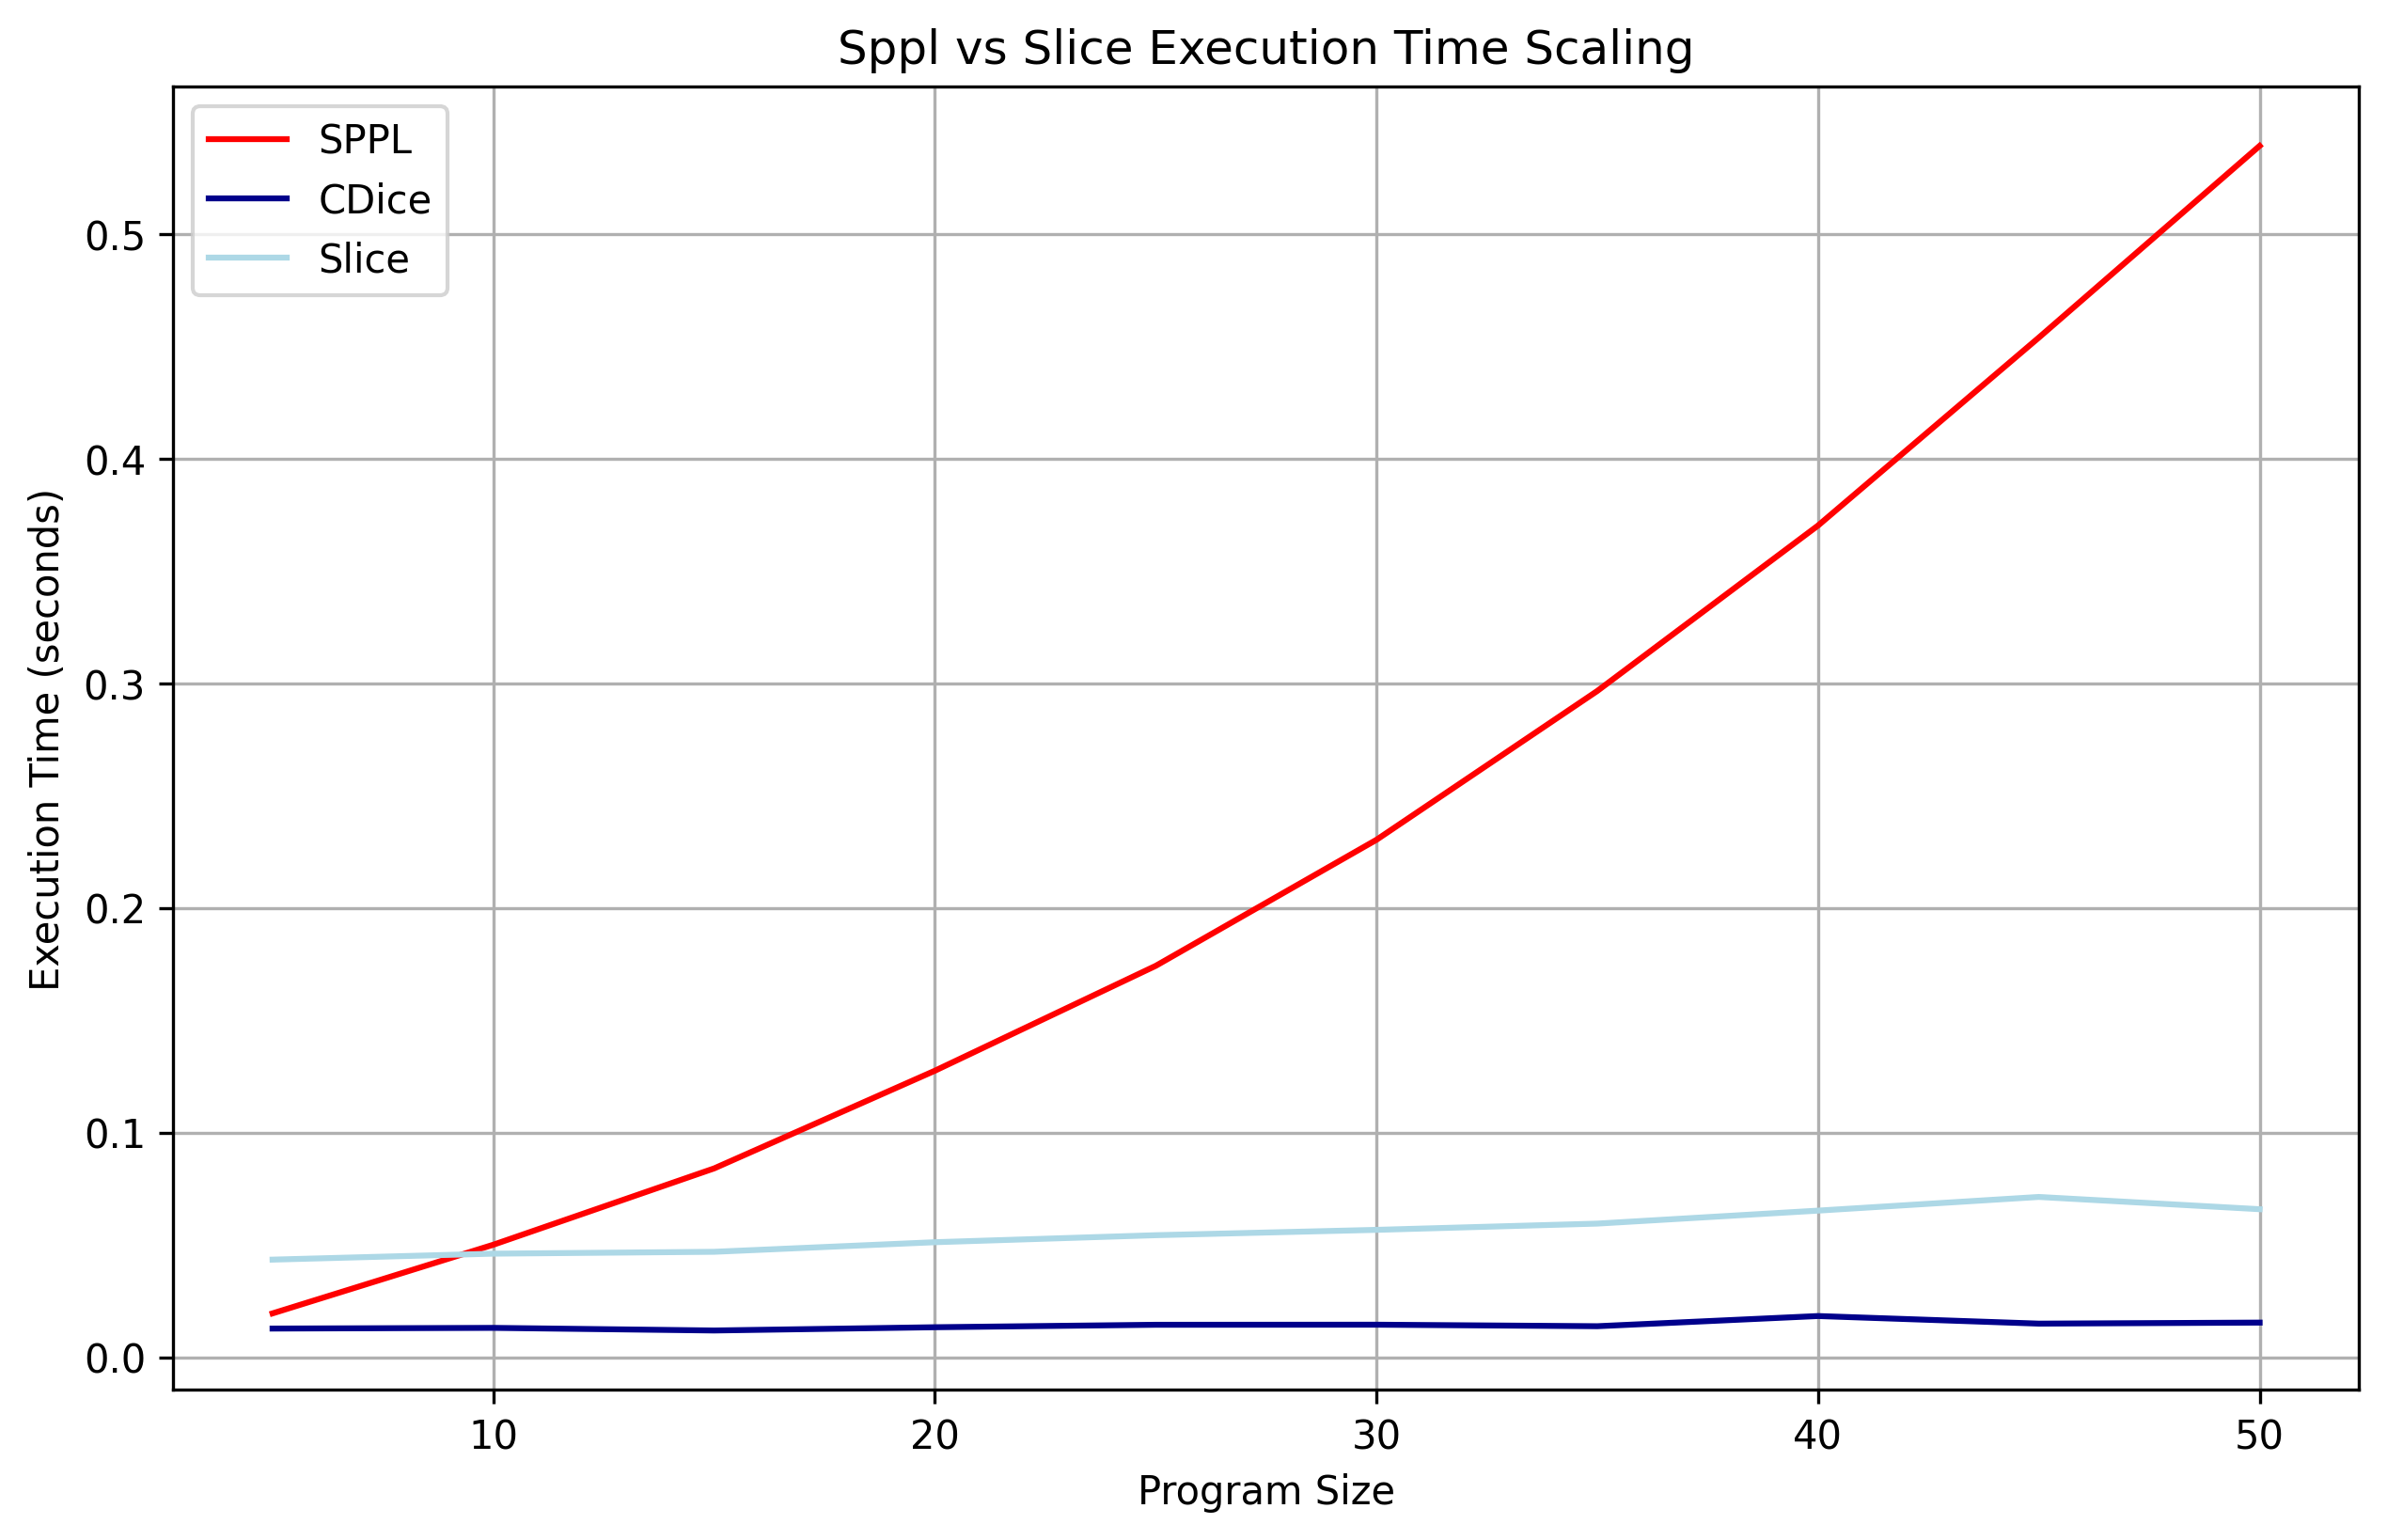
\includegraphics[width=\textwidth]{../images/scaling/build_alternating_guard_contdice_2.png}
\caption{Alternating Guard 2}
\end{subfigure}
\vspace{0.5em}
\begin{subfigure}{0.48\textwidth}
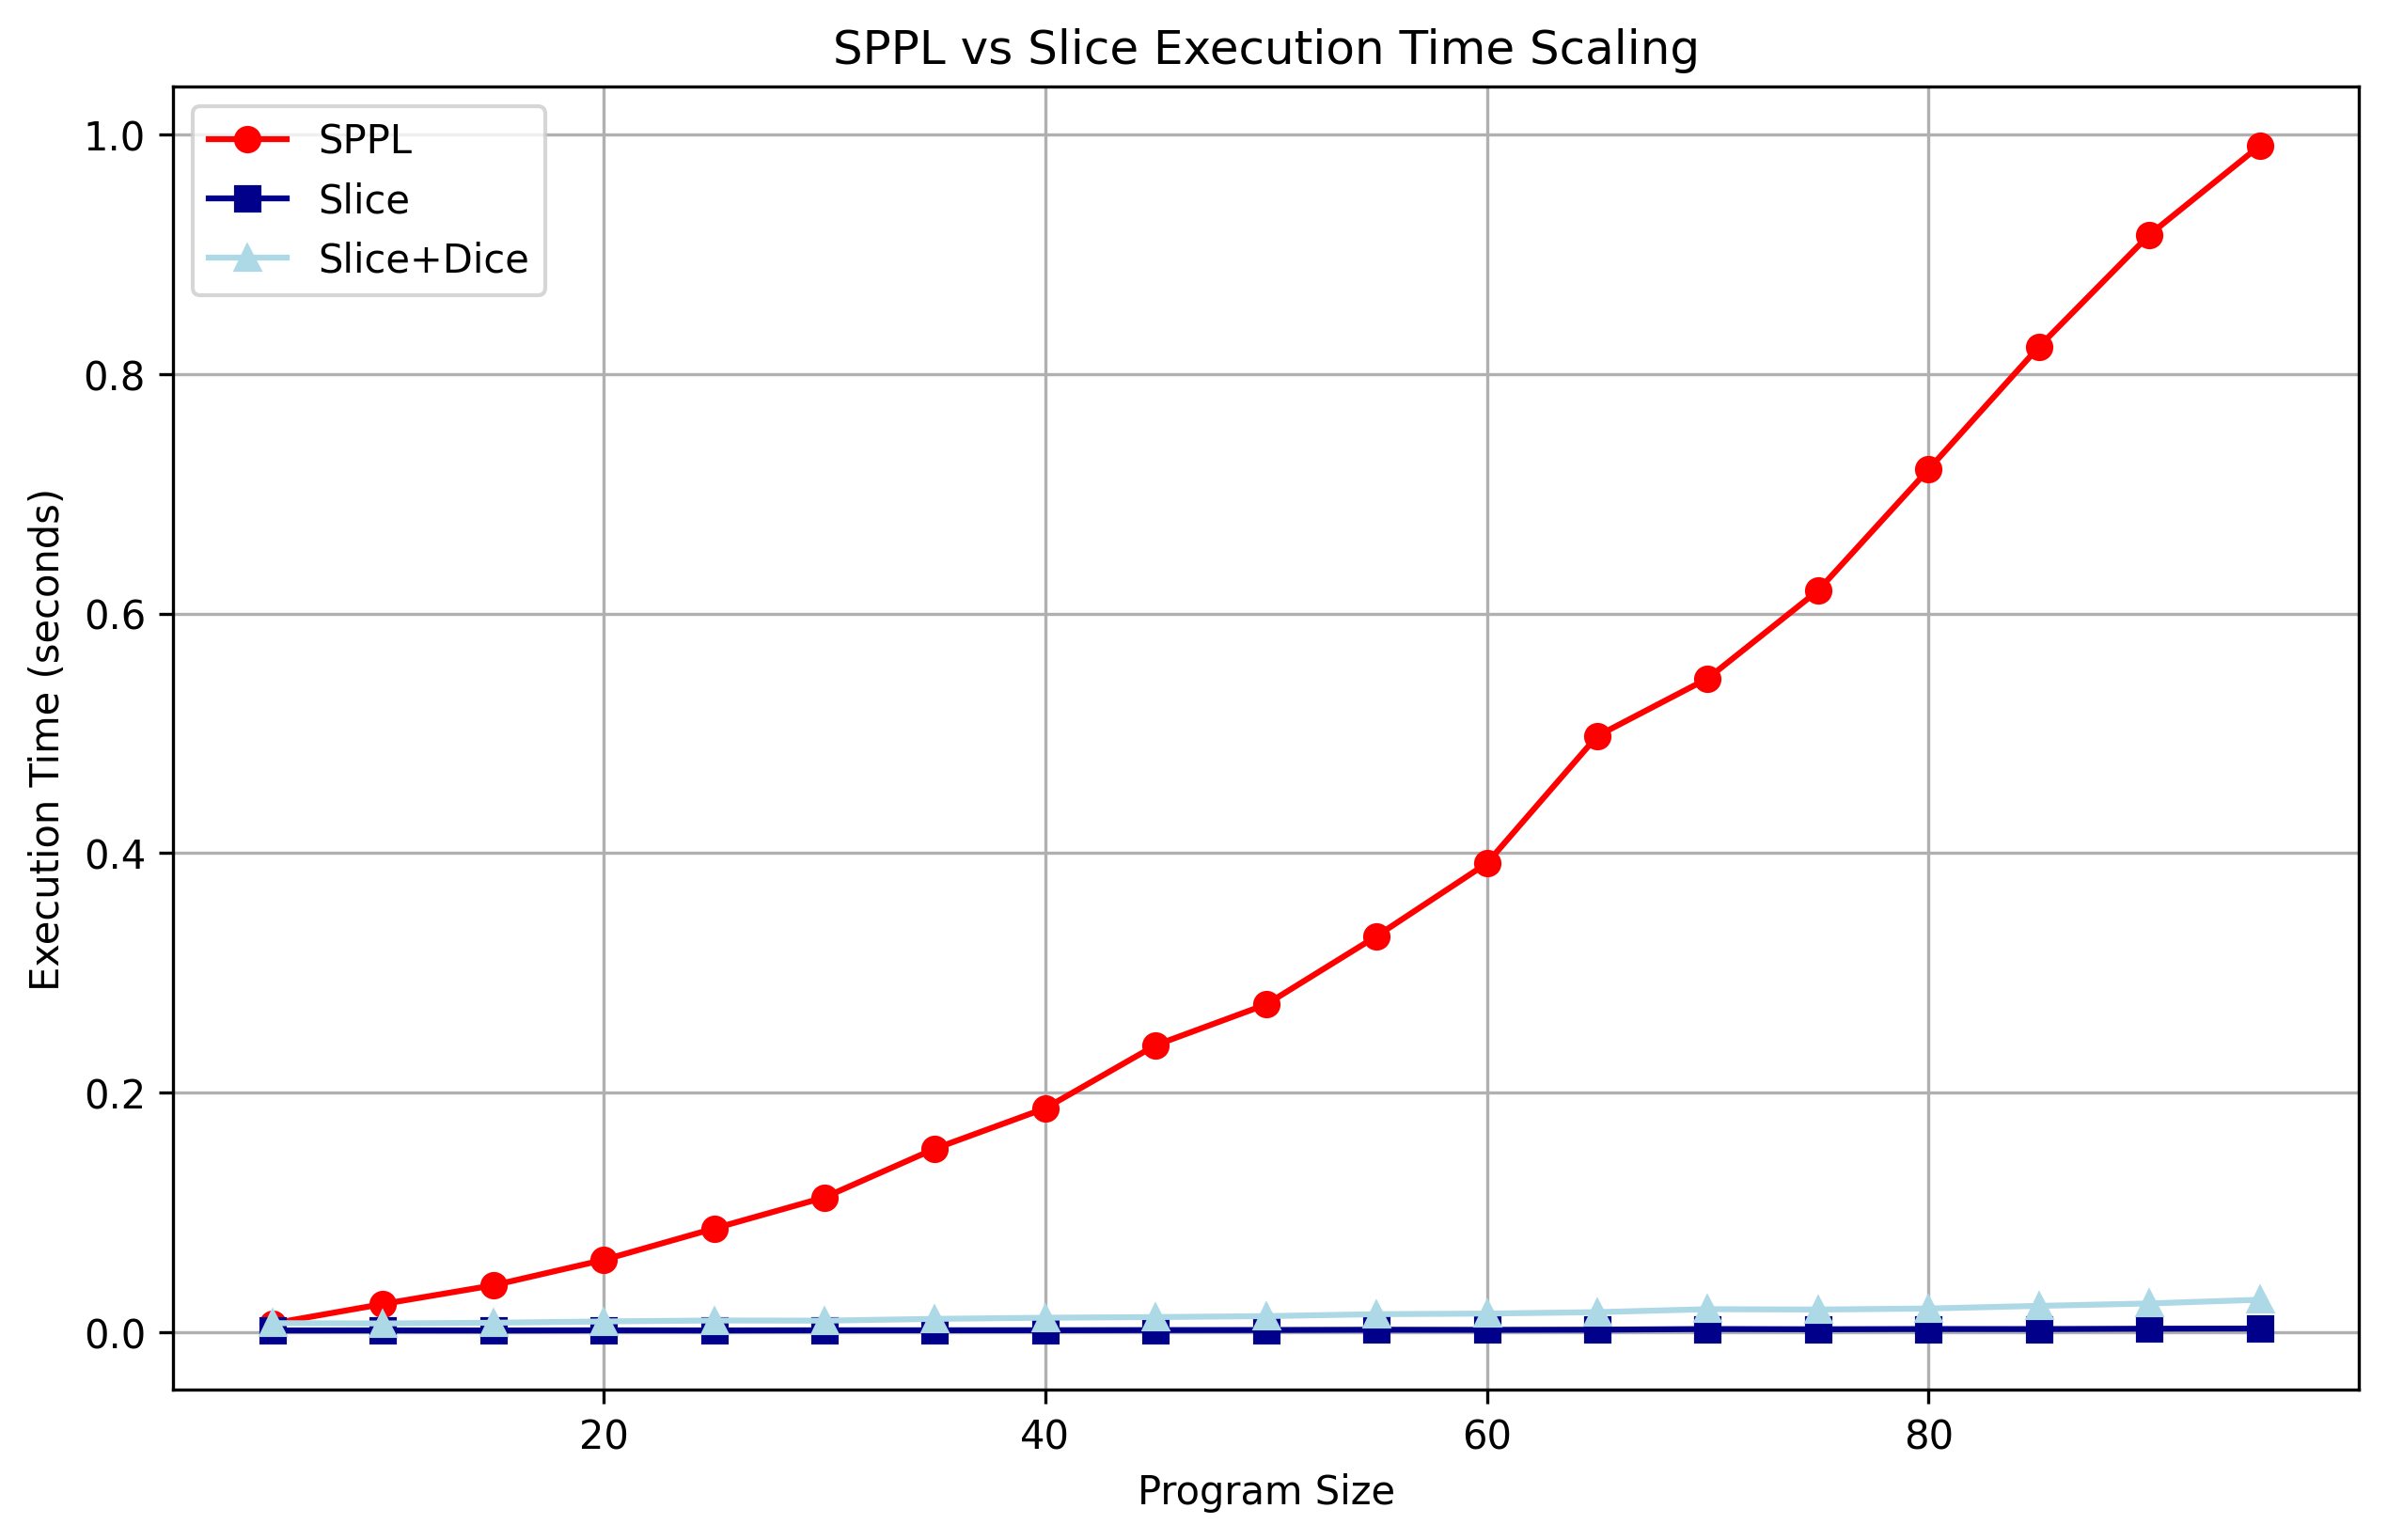
\includegraphics[width=\textwidth]{../images/scaling/build_alternating_guard_contdice_3.png}
\caption{Alternating Guard 3}
\end{subfigure}
\hfill
\begin{subfigure}{0.48\textwidth}
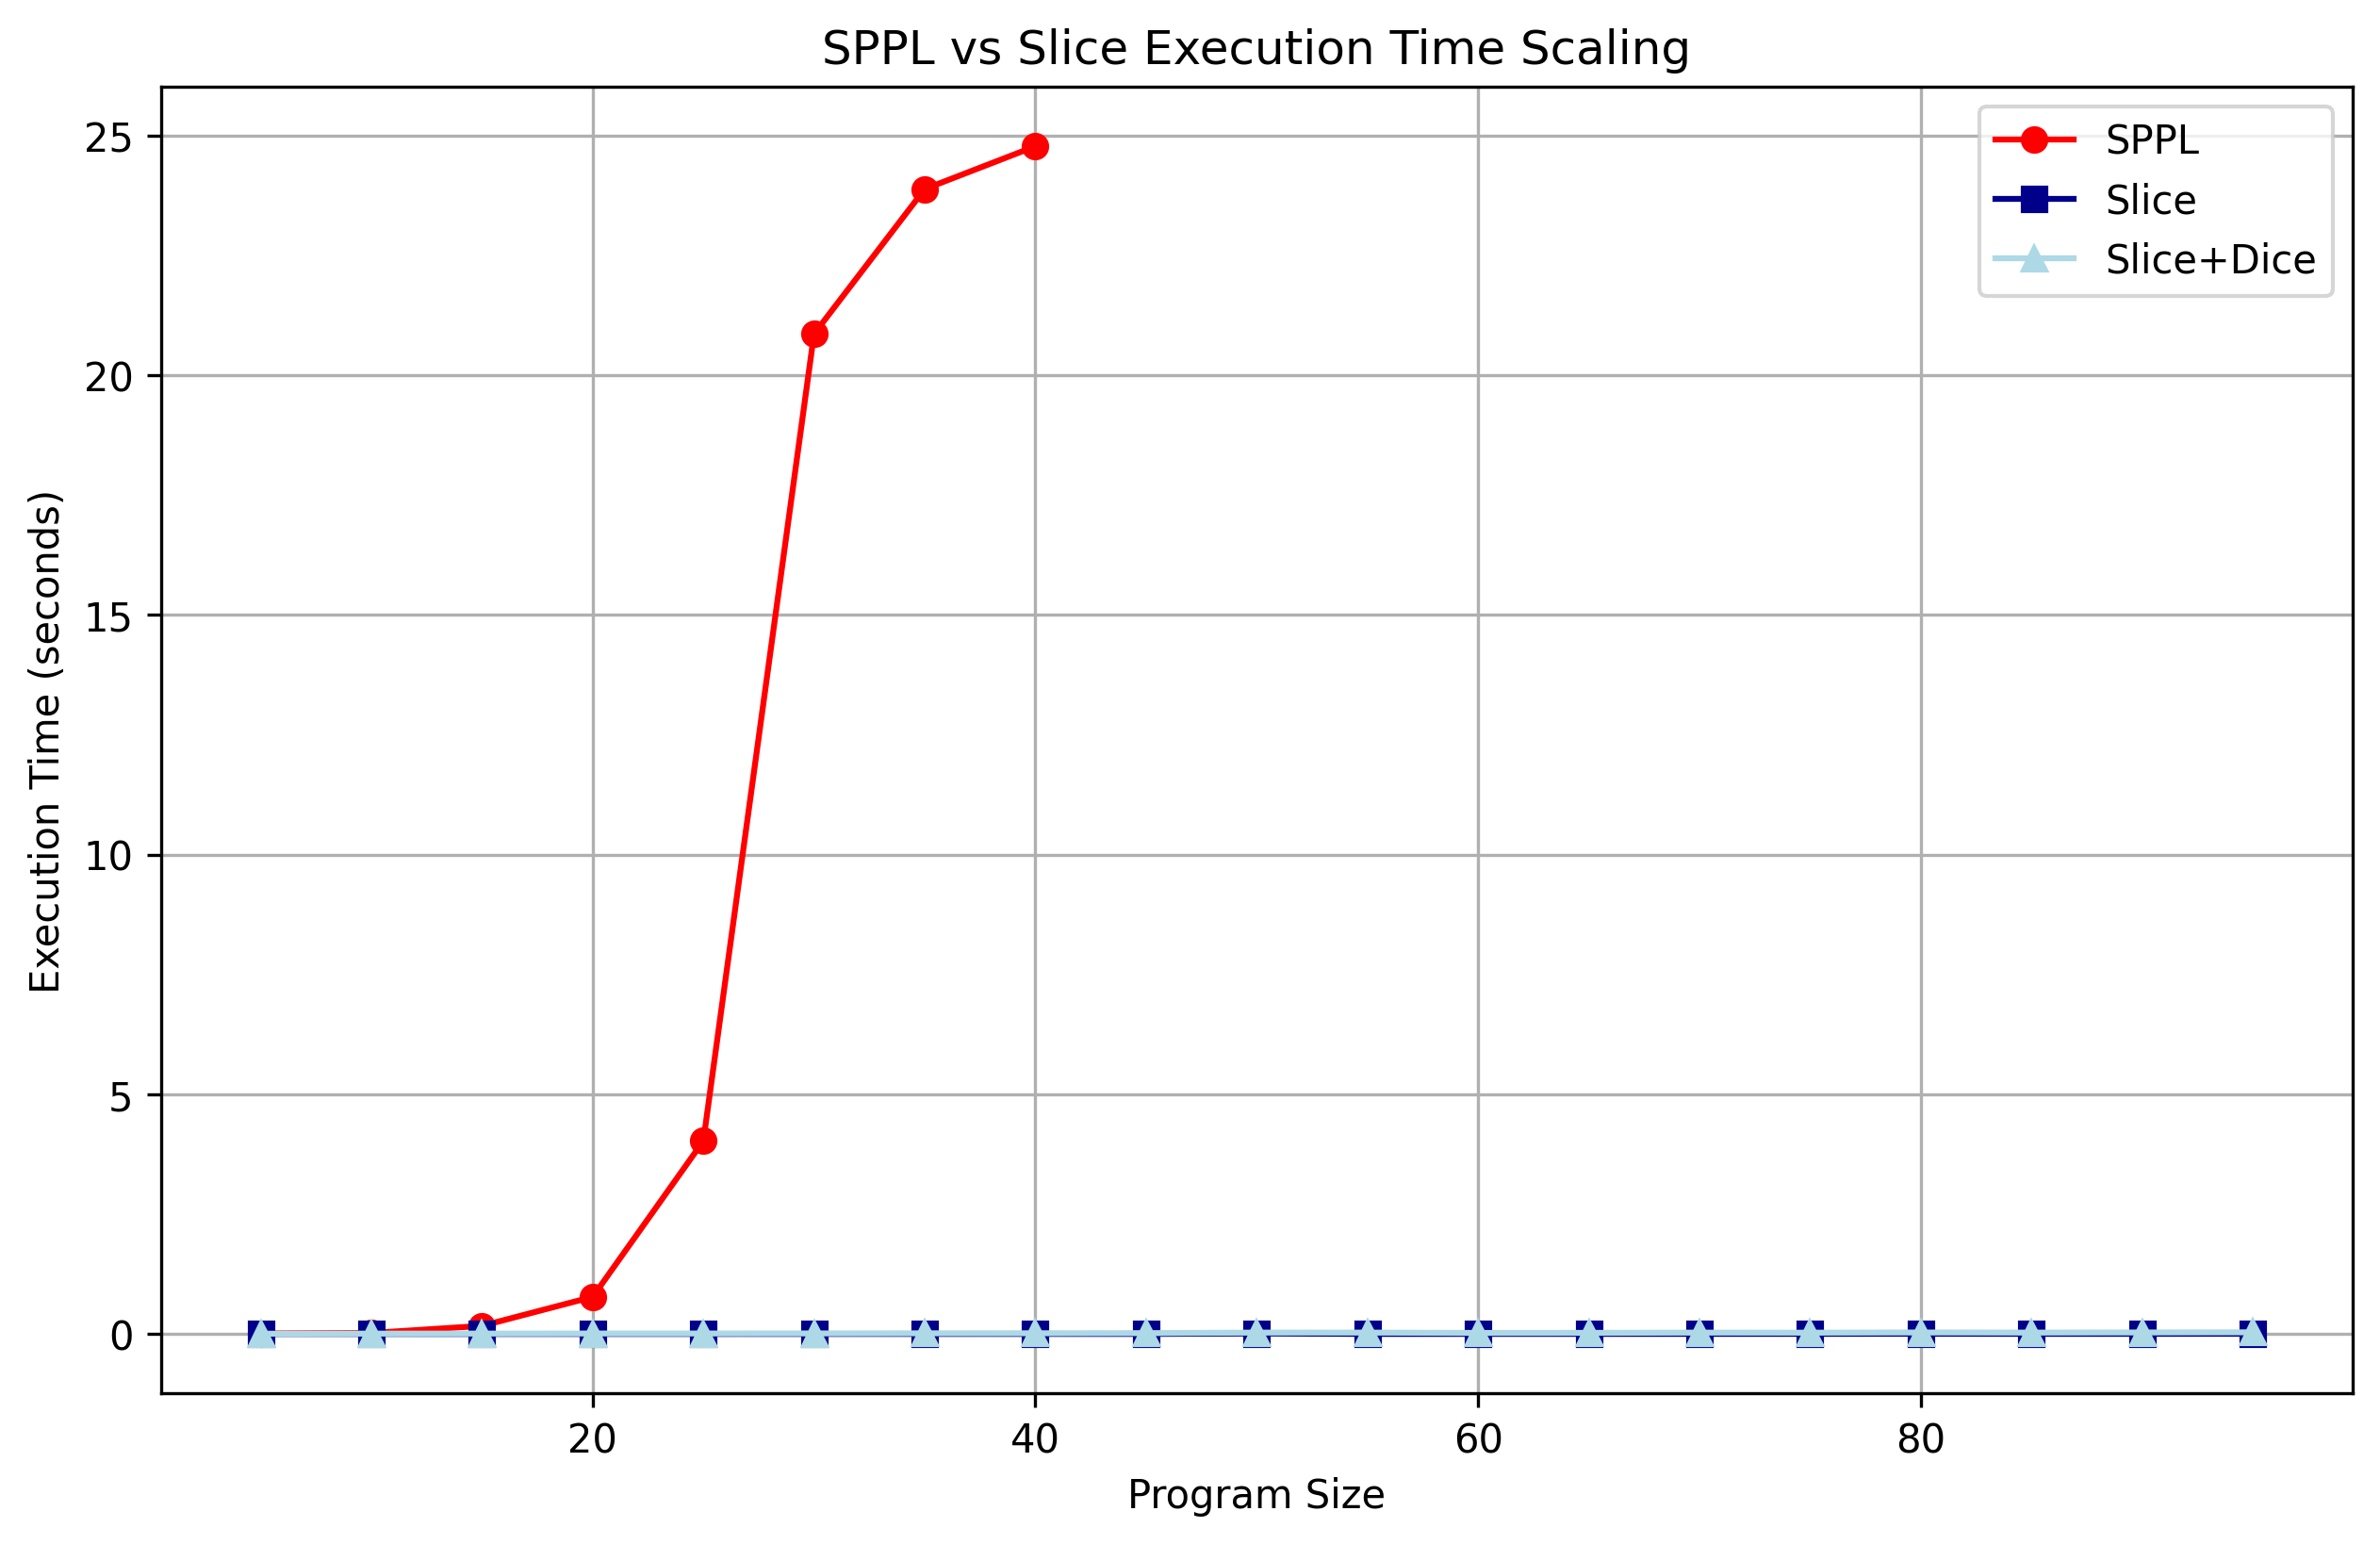
\includegraphics[width=\textwidth]{../images/scaling/build_random_alternating_guard_contdice.png}
\caption{Random Alternating Guard}
\end{subfigure}
\caption{Scaling results for alternating guard benchmarks. SPPL (red) times out early (between program sizes 20-30), while Slice continues to scale to large programs.}
\label{fig:alt-benchmarks}
\end{figure}